%%%
% Plantilla de Trabajo
% Modificación de una plantilla de Latex de Frits Wenneker para adaptarla 
% al castellano y a las necesidades de escribir informática y matemáticas.
%
% Editada por: Mario Román
%
% License:
% CC BY-NC-SA 3.0 (http://creativecommons.org/licenses/by-nc-sa/3.0/)
%%%

%%%%%%%%%%%%%%%%%%%%%%%%%%%%%%%%%%%%%%%%
% Short Sectioned Assignment
% LaTeX Template
% Version 1.0 (5/5/12)
%
% This template has been downloaded from:
% http://www.LaTeXTemplates.com
%
% Original author:
% Frits Wenneker (http://www.howtotex.com)
%
% License:
% CC BY-NC-SA 3.0 (http://creativecommons.org/licenses/by-nc-sa/3.0/)
%
%%%%%%%%%%%%%%%%%%%%%%%%%%%%%%%%%%%%%%%%%

%----------------------------------------------------------------------------------------
%	PAQUETES Y CONFIGURACIÓN DEL DOCUMENTO
%----------------------------------------------------------------------------------------

%%% Configuración del papel.
% fourier: Usa la fuente Adobe Utopia. (Comentando la línea usa la fuente normal)
\documentclass[paper=a4, fontsize=11pt, spanish]{scrartcl} 
\usepackage{fourier}

% Centra y formatea los títulos de sección.
% Quita la indentación de párrafos.
\usepackage{sectsty} % Allows customizing section commands
\allsectionsfont{\centering \normalfont\scshape} % Make all sections centered, the default font and small caps
\setlength\parindent{0pt} % Removes all indentation from paragraphs - comment this line for an assignment with lots of text

% Permite elegir cabeceras y pies de página.
\usepackage{fancyhdr} % Custom headers and footers
\pagestyle{fancyplain} % Makes all pages in the document conform to the custom headers and footers
\fancyhead{} % No page header - if you want one, create it in the same way as the footers below
\fancyfoot[L]{} % Empty left footer
\fancyfoot[C]{} % Empty center footer
\fancyfoot[R]{\thepage} % Page numbering for right footer
\renewcommand{\headrulewidth}{0pt} % Remove header underlines
\renewcommand{\footrulewidth}{0pt} % Remove footer underlines
\setlength{\headheight}{13.6pt} % Customize the height of the header


%%% Castellano.
% noquoting: Permite uso de comillas no españolas.
% lcroman: Permite la enumeración con numerales romanos en minúscula.
% fontenc: Usa la fuente completa para que pueda copiarse correctamente del pdf.
\usepackage[spanish,es-noquoting,es-lcroman]{babel}
\usepackage[utf8]{inputenc}
\usepackage[T1]{fontenc}
\selectlanguage{spanish}


%%% Matemáticas.
% Paquetes de la AMS. Para entornos de ecuaciones.
\usepackage{amsmath,amsfonts,amsthm}

% Incluye números entre secciones y ecuaciones.
\numberwithin{equation}{section} % Number equations within sections (i.e. 1.1, 1.2, 2.1, 2.2 instead of 1, 2, 3, 4)
\numberwithin{figure}{section} % Number figures within sections (i.e. 1.1, 1.2, 2.1, 2.2 instead of 1, 2, 3, 4)
\numberwithin{table}{section} % Number tables within sections (i.e. 1.1, 1.2, 2.1, 2.2 instead of 1, 2, 3, 4)

%%% Códigos C / C++ / SQL ...
% Paquete listings para visualización de código más elegante
\usepackage{xcolor,listings}
\usepackage{textcomp}
\lstset{upquote=true}

%% Gráficos e imagenes:
\usepackage{graphicx}


%----------------------------------------------------------------------------------------
%	TÍTULO
%----------------------------------------------------------------------------------------
% Título con las líneas horizontales, nombres y fecha.

\newcommand{\horrule}[1]{\rule{\linewidth}{#1}} % Create horizontal rule command with 1 argument of height

\title{
  \normalfont \normalsize 
  \textsc{Universidad de Granada.\\Sistemas Multidimensionales} \\ [25pt] % Your university, school and/or department name(s)
  \horrule{0.5pt} \\[0.4cm] % Thin top horizontal rule
  \huge Práctica 2: Implementación de esquemas de bases de datos multidimensionales I \\ % The assignment title
  \horrule{2pt} \\[0.5cm] % Thick bottom horizontal rule
}

\author{Daniel López García\\Rafael Nogales Vaquero} % Your name

\date{\normalsize\today} % Today's date or a custom date



%----------------------------------------------------------------------------------------
%	DOCUMENTO
%----------------------------------------------------------------------------------------


\begin{document}
\maketitle % Escribe el título

En primer lugar para obtener la tabla de la dimensión Fecha, hacemos una consulta de las fechas, obteniendo el año de las mismas.
\begin{lstlisting}[
language=SQL,
breaklines=true,
showspaces=false,
basicstyle=\ttfamily,
numbers=left,
numberstyle=\tiny,
commentstyle=\color{gray}
]
SELECT DISTINCT LineaDeVenta.Fecha,Year([LineaDeVenta].[Fecha]) AS Anio INTO Fecha 
FROM LineaDeVenta;

\end{lstlisting}
Podemos ver el resultado de la ejecución de la consulta en las siguientes imagen:\\
\\
\begin{center}
	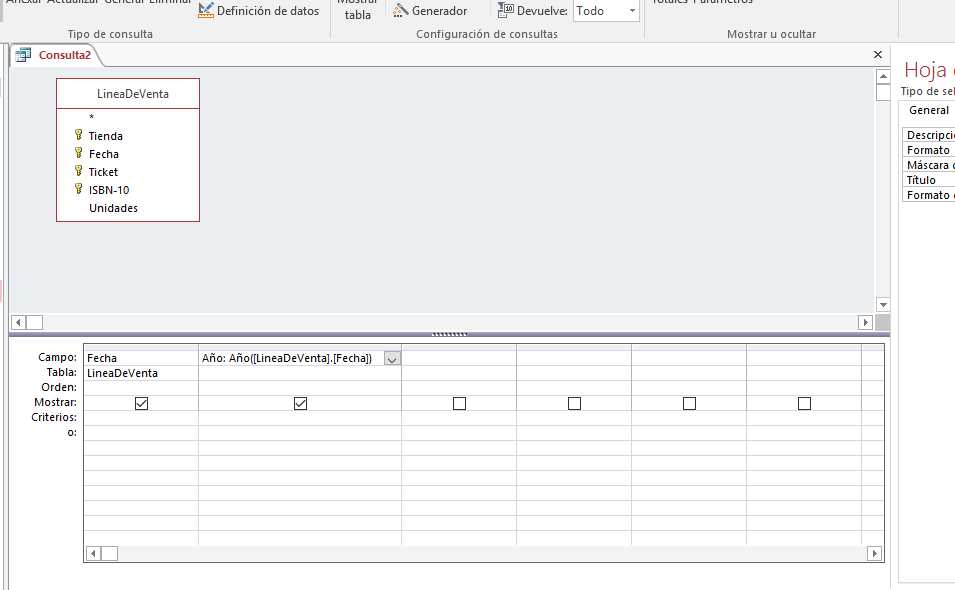
\includegraphics[scale=0.35]{fecha1.png}
	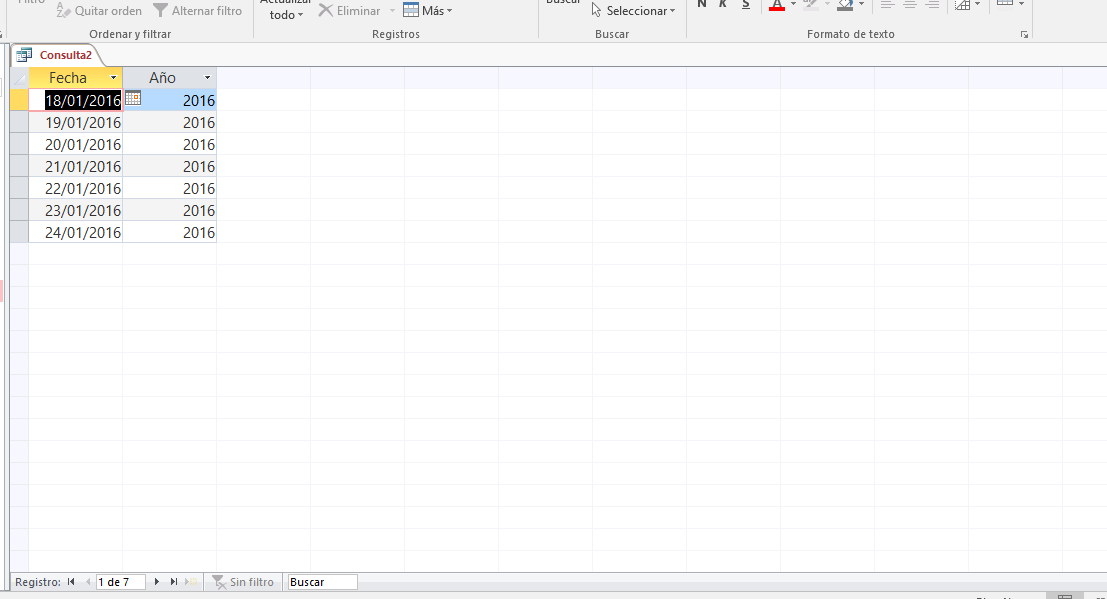
\includegraphics[scale=0.35]{fecha2.png}
\end{center}

A continuación, efectuamos las agregaciones en la tabla LineaDeVenta
\begin{lstlisting}[
language=SQL,
breaklines=true,
showspaces=false,
basicstyle=\ttfamily,
numbers=left,
numberstyle=\tiny,
commentstyle=\color{gray}
]
SELECT LineaDeVenta.Tienda, LineaDeVenta.[ISBN-10], LineaDeVenta.Fecha, Sum(LineaDeVenta.Unidades) AS Unidades_, Count(LineaDeVenta.Ticket) AS Clientes, Sum([PVP]*[Unidades]) AS Importe, [Importe]/Sum([Unidades]) AS Media_precio INTO aux
FROM Libro LEFT JOIN LineaDeVenta ON Libro.[ISBN-10] = LineaDeVenta.[ISBN-10]
GROUP BY LineaDeVenta.Tienda, LineaDeVenta.[ISBN-10], LineaDeVenta.Fecha;

\end{lstlisting}
\begin{center}
	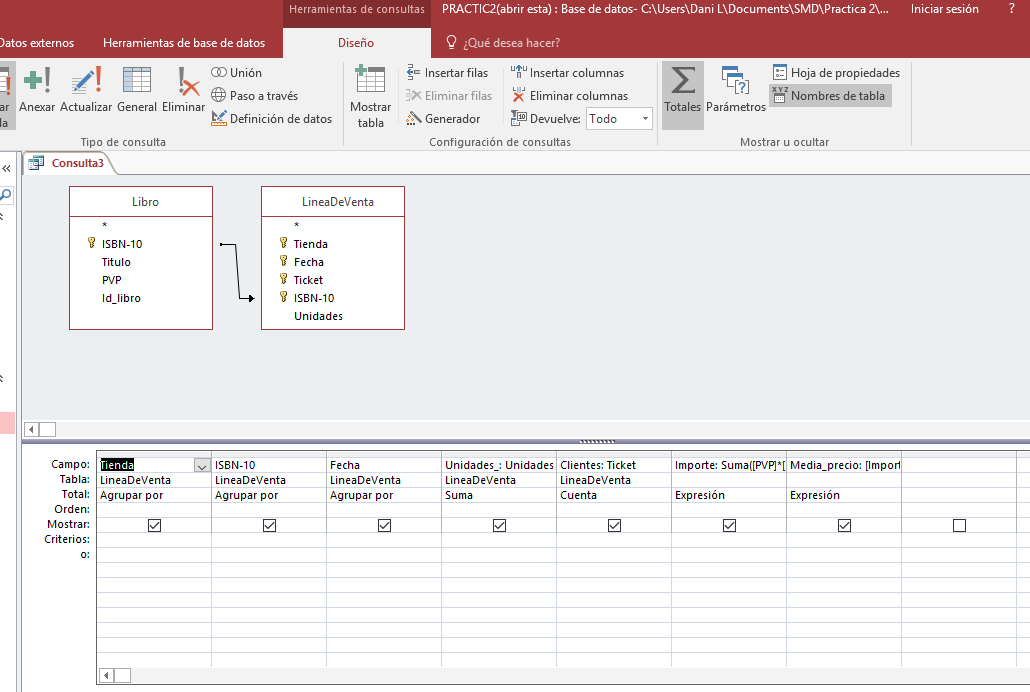
\includegraphics[scale=0.35]{sum1.png}
	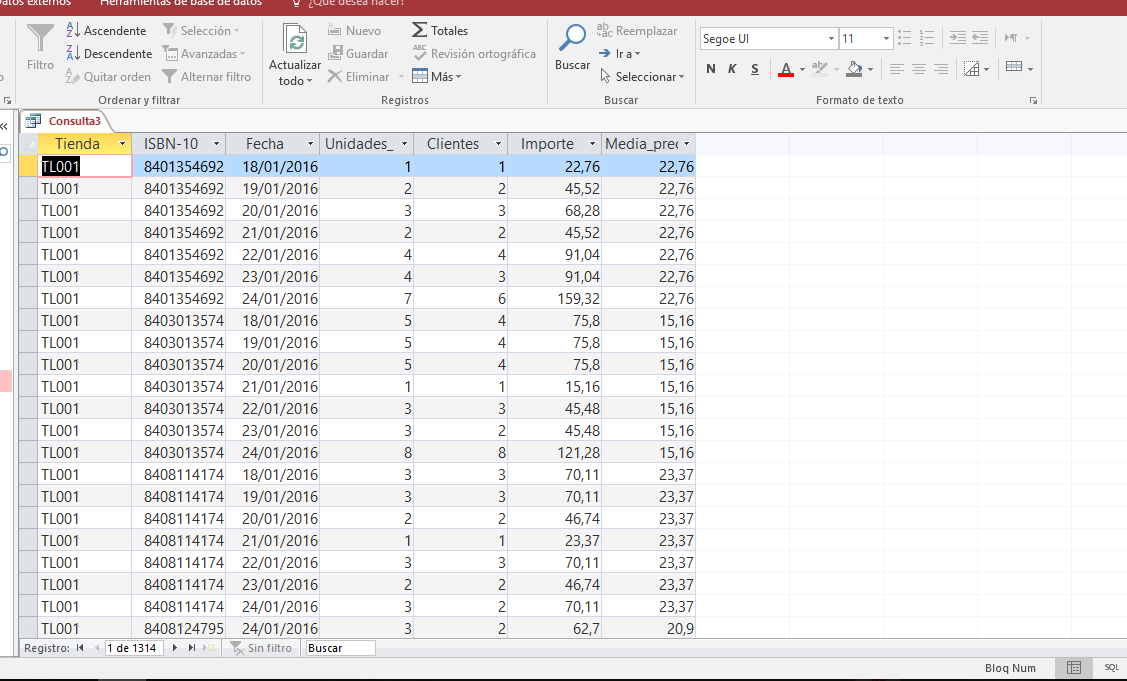
\includegraphics[scale=0.35]{sum2.png}
\end{center}
Y finalmente, cambiamos los códigos por los identificadores
\begin{lstlisting}[
language=SQL,
breaklines=true,
showspaces=false,
basicstyle=\ttfamily,
numbers=left,
numberstyle=\tiny,
commentstyle=\color{gray}
]
SELECT Libro.Id_libro, Fecha.Id_fecha, Tienda.Id_tienda, aux.Unidades_, aux.Clientes, aux.Importe, aux.Media_precio INTO Venta
FROM Fecha INNER JOIN (Tienda INNER JOIN (aux INNER JOIN Libro ON aux.[ISBN-10] = Libro.[ISBN-10]) ON Tienda.Cod_tienda = aux.Tienda) ON Fecha.Fecha = aux.Fecha
WHERE (((aux.[ISBN-10])=[Libro].[ISBN-10]) AND ((aux.Fecha)=[Fecha].[Fecha]) AND ((aux.Tienda)=[Tienda].[Cod_tienda]));


\end{lstlisting}
\begin{center}
	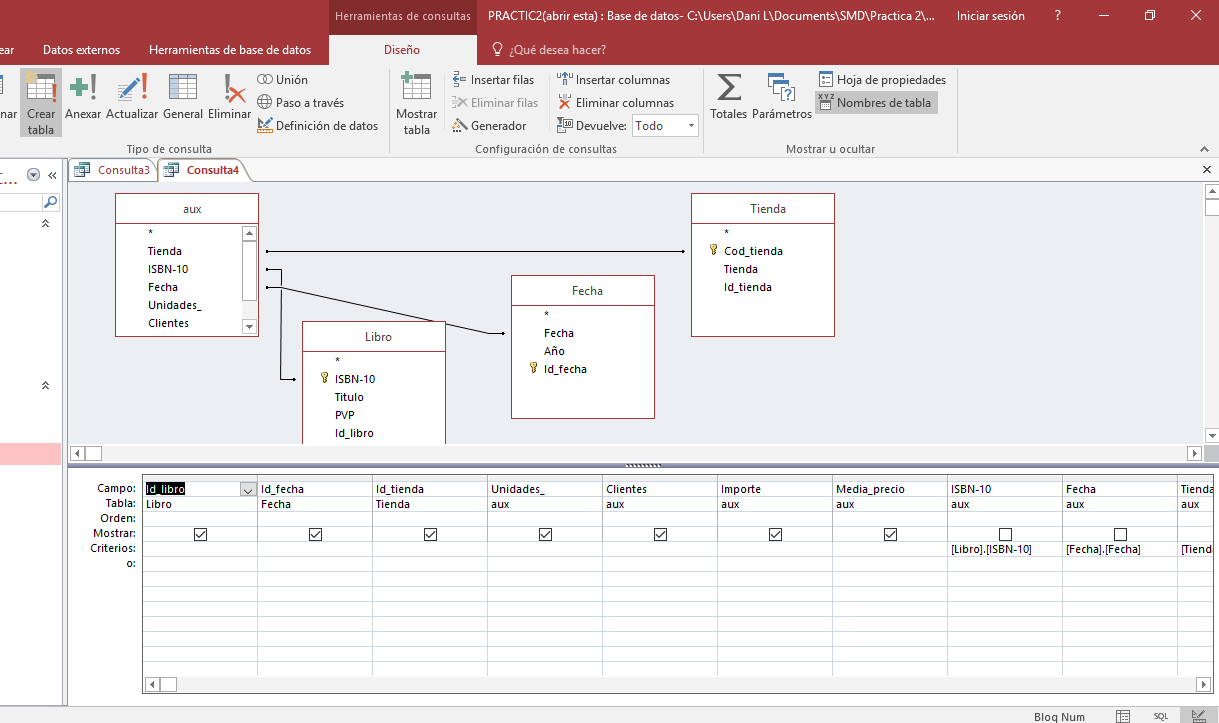
\includegraphics[scale=0.35]{id1.png} \\
	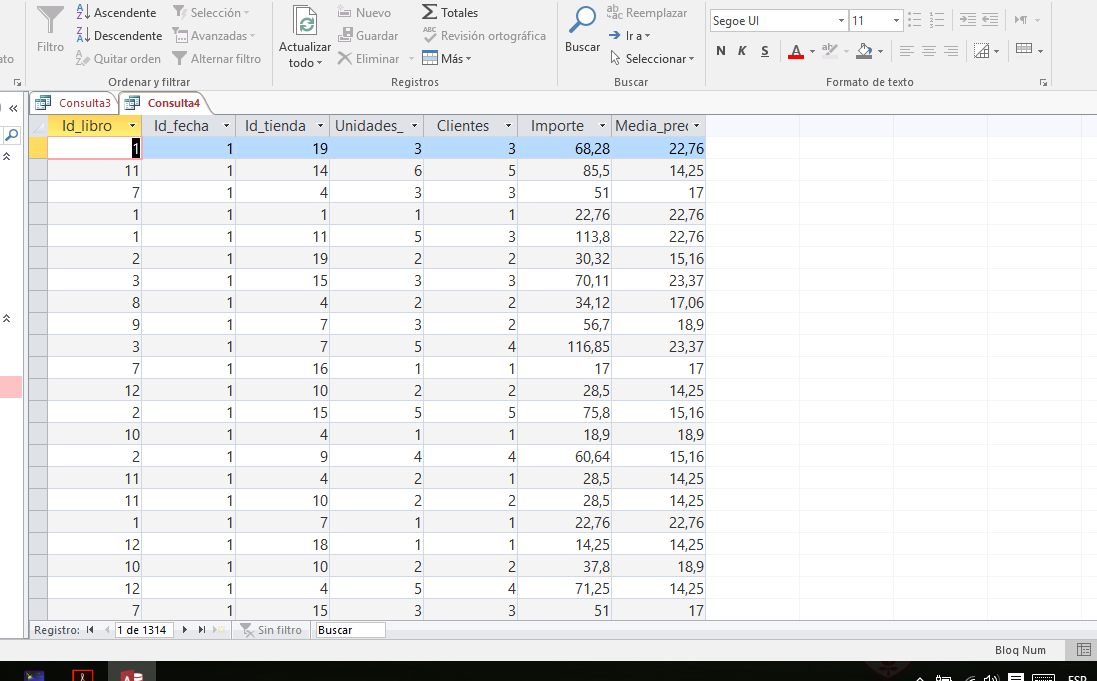
\includegraphics[scale=0.35]{id2.png}
\end{center}

\end{document}